\documentclass[a4paper, twocolumn]{article}
\usepackage{lipsum}
\usepackage{marvosym}
\usepackage{graphicx}
\usepackage{subcaption}
\usepackage{tikz}

\title{Fundamentals Of \LaTeX}
\author{BATIKAN BORA ORMANCI}

\begin{document}
	\maketitle	
	
	\begin{abstract}
		\lipsum[1]
	\end{abstract}
	
	\tableofcontents
	
	\section{Introduction}
	In Ipsum in Section \ref{sec:ipsum} we will discuss x, y and z. 
	\subsection{a subsection}
	\lipsum
	\subsubsection{A subsubsection}\label{sec:ipsum}
	
	\subsection{another subsection}
	\lipsum[1]
	
	\paragraph{Short Point}
	This is a small point. This is 
	a sentence which is still part of the same paragraph. 
	
	This is a new paragraph. 
	
	\section{Basic Typesetting}
	\subsection{Symbols}
	\EUR \EURhv
	
	\subsection{Accents}
	\"{a}\H{b}\.{c}\'{e}\`{e}\^{e}\v{e}\u{e}\={e}
	
	\subsection{Emphasis}
	\textbf{boldface text.}
	Normal text.
	\textit{italic text.}
	Combining multiple of them \textbf{\textit{within}} a sentence. 
	
	{\tt Text in typewriter font.}
	
	\subsection{Font Sizes}
	{\tiny tiny text} \\
	\begin{normalsize}
		normal-sized text. \\
	\end{normalsize}
	\begin{huge}
		huge text.
	\end{huge}
	
	normal-sized text. 
	
	\subsection{Quotations}
	As seen in this quote:
	
	\begin{quote}
		Next to the originator of a good sentence
		is the first quoter of it. \\
		\textit{- Ralph Waldo Emerson}
	\end{quote}
	
		\begin{figure}
		\begin{subfigure}{0.25\textwidth} % Default Options: tbp
			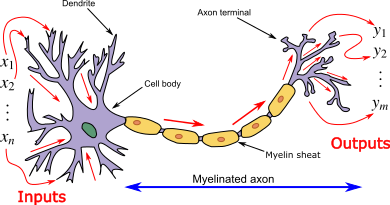
\includegraphics[width=\linewidth]{Figures/bio-neuron.png}
			\caption{This is a biological neuron}
			\label{fig:bio-neur2}
		\end{subfigure}
		
		\begin{subfigure}{0.25\textwidth}
			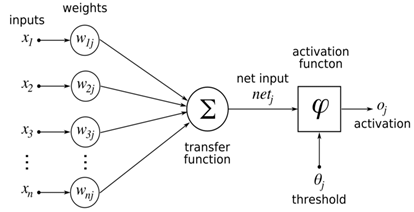
\includegraphics[width=\linewidth]{Figures/artificial-neuron.png}
			\caption{This is an artificial neuron}
			\label{fig:artificial-neuron2}
		\end{subfigure}
	\end{figure}
	
	\section{Lists}
	\subsection{Ordered Lists}
	\begin{enumerate}
		\item First
		\item Second
		\item Third
		\begin{enumerate}
			\item Bread
			\item Milk
		\end{enumerate}
	\end{enumerate}
	
	\subsection{Unordered List}
	\begin{itemize}
		\item Bread
		\item Milk
		\item Cheese
		\begin{enumerate}
			\item First
			\item Second
		\end{enumerate}
	\end{itemize}
	
	\section{Plots}
	\begin{tikzpicture}
		\draw (0, 0) rectangle (0.4, 0.2);
	\end{tikzpicture}
	
	
\begin{tikzpicture}[scale=10]
		\draw (0, 0) rectangle (0.4, 0.2);
		\draw (0, 0) -- (0.4, 0.2);
	\end{tikzpicture}	
	
	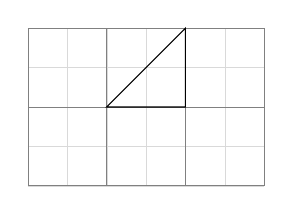
\begin{tikzpicture}[scale=1]
		\draw[line width=0.1pt, gray!30, step=5mm] (0,0) grid (3,2);
		\draw[help lines] (0,0) grid (3,2);
		\draw (1,1) -- (2,2) -- (2,1) -- cycle;

	\end{tikzpicture}	
	% You could also put tikz graphics into figure environments to add captions etc

	\appendix
	\section{Derivations}
	Here we derive Formula 3.2...
	
	\section{Additional Figures}
	
	
\end{document}
















